\documentclass[12pt]{article}
\setlength{\oddsidemargin}{0.25 in}
\setlength{\evensidemargin}{-0.25 in}
\setlength{\topmargin}{-0.6 in}
\setlength{\textwidth}{6.5 in}
\setlength{\textheight}{8.5 in}
\setlength{\headsep}{0.75 in}
\setlength{\parindent}{0 in}
\setlength{\parskip}{0.1 in}

%
% ADD PACKAGES here:
%

\usepackage{amsmath,amsfonts,amssymb,graphicx,mathtools}
\usepackage{multirow,url}

%
% The following commands set up the lecnum (lecture number)
% counter and make various numbering schemes work relative
% to the lecture number.
%
\newcounter{lecnum}
\renewcommand{\thepage}{\thelecnum-\arabic{page}}
\renewcommand{\thesection}{\thelecnum.\arabic{section}}
\renewcommand{\theequation}{\thelecnum.\arabic{equation}}
\renewcommand{\thefigure}{\thelecnum.\arabic{figure}}
\renewcommand{\thetable}{\thelecnum.\arabic{table}}

%
% The following macro is used to generate the header.
%
\newcommand{\lecture}[4]{
   \pagestyle{myheadings}
   \thispagestyle{plain}
   \newpage
   \setcounter{lecnum}{#1}
   \setcounter{page}{1}
   \noindent
   \begin{center}
   	\framebox{
   		\vbox{\vspace{2mm}
   			\hbox to 6.28in { {\bf MATH 254: Introduction to Statistics
   					\hfill #3} }
   			\vspace{4mm}
   			\hbox to 6.28in { {\Large \hfill Lesson #1: #2  \hfill} }
   			\vspace{2mm}
   			\hbox to 6.28in { {\hfill Corresponding Workbook Module: #4} }
   			\vspace{2mm}}
   	}
   \end{center}
   \markboth{Handout #1}{Handout #1}

   %{\bf Note}: {\it LaTeX template courtesy of UC Berkeley EECS dept.}

   %{\bf Disclaimer}: {\it These notes have not been subjected to the usual scrutiny reserved for formal publications.  They may be distributed outside this class only with the permission of the instructor.}
   %\vspace*{4mm}
   \vspace*{-4mm}
}
%
% Convention for citations is authors' initials followed by the year.
% For example, to cite a paper by Leighton and Maggs you would type
% \cite{LM89}, and to cite a paper by Strassen you would type \cite{S69}.
% (To avoid bibliography problems, for now we redefine the \cite command.)
% Also commands that create a suitable format for the reference list.
\renewcommand{\cite}[1]{[#1]}
\def\beginrefs{\begin{list}%
        {[\arabic{equation}]}{\usecounter{equation}
         \setlength{\leftmargin}{2.0truecm}\setlength{\labelsep}{0.4truecm}%
         \setlength{\labelwidth}{1.6truecm}}}
\def\endrefs{\end{list}}
\def\bibentry#1{\item[\hbox{[#1]}]}

%Use this command for a figure; it puts a figure in wherever you want it.
%usage: \fig{NUMBER}{SPACE-IN-INCHES}{CAPTION}
\newcommand{\fig}[3]{
			\vspace{#2}
			\begin{center}
			Figure \thelecnum.#1:~#3
			\end{center}
	}
% Use these for theorems, lemmas, proofs, etc.
\newtheorem{example}{Example}[lecnum]
\newtheorem{exercise}{Exercise}[lecnum]

\newtheorem{theorem}{Theorem}[lecnum]
\newtheorem{definition}[theorem]{Definition}
\newenvironment{proof}{{\bf Proof:}}{\hfill\rule{2mm}{2mm}}

% **** IF YOU WANT TO DEFINE ADDITIONAL MACROS FOR YOURSELF, PUT THEM HERE:

\newcommand\E{\mathbb{E}}

\begin{document}
%FILL IN THE RIGHT INFO.
%\lecture{**LECTURE-NUMBER**}{**DATE**}{**LECTURER**}{**SCRIBE**}
\lecture{4}{Inference for a Difference in Two Means}{Mintaek Lee}{5}
%\footnotetext{These notes are partially based on those of Nigel Mansell.}

% **** YOUR NOTES GO HERE:
\begin{example}	Hypothesis testing for a paired (dependent) sample \\
	Mintaek wants to know if there is a difference between population mean Exam 1 scores and population mean Exam 2 scores of his students. He randomly selected 7 students across his classes and collected their \mbox{Exam 1 }and Exam 2 scores. Use the appropriate statistical methods and set up the hypotheses that best match Mintaek's interests.
	\begin{table}[!h]
		\centering
		\begin{tabular}{l|lllllll}
			Student & 1  & 2  & 3  & 4  & 5  & 6  & 7  \\ \hline
			Exam 1  & 77 & 70 & 86 & 72 & 92 & 62 & 69 \\
			Exam 2  & 81 & 79 & 83 & 82 & 98 & 60 & 76
		\end{tabular}
	\end{table}
\end{example}
\vspace{-20pt}

You first need to recognize that this is a paired sample. It is because each observation in Exam 1 can be paired with one in Exam 2 since both scores came from the same student. In general, you can say that you have a paired data when you can match each individual observation from one group to another from the other group (like in matched pairs experiment or matched pairs observational study). You can match them when they have something in common. For example, when you have two observations from a same person or two people with similar characteristics. 

We use the paired t-test for this problem since we have a paired data. When we are working with the paired data, we only concern ourselves with the differences between two exam scores within each pair. In fact, we will not even be considering the original data anymore.

\begin{table}[!h]
	\centering
	\begin{tabular}{l|lllllll}
		Student & 1  & 2  & 3  & 4  & 5  & 6  & 7  \\ \hline
		Difference & -4  & -9  & 3  & -10  & -6  & 2  & -7
	\end{tabular}
\end{table}

Using software, we find $\bar{x}_D = -4.43857$ (sample mean of differences), ${s_D = 5.12696}$ (sample standard deviation of differences), and $n = 7$ (sample size). Note that the sample size is obtained by counting the number of pairs for the paired t-test, NOT the total number of test scores.

\noindent \textbf{Step 1}: Since the problem did not explicitly specify how much of a difference we want to see, any difference larger than 0 would suffice for our testing. In this case, any significant difference will do.
\begin{itemize}
	\item $H_0$: $\mu_D = 0$, population mean difference in exam scores is \textbf{equal to} 0.
	\item $H_A$: $\mu_D \neq 0$, population mean difference in exam scores is \textbf{different from} 0.
\end{itemize}

\noindent \textbf{Step 2}: We are using the matched paires t-test here (matched pairs t-test and paired t-test mean the same thing). We check all the underlying conditions (See workbook page 149 then 91 for the description of conditions). For the significance level, we will use $\alpha = 0.05$.

We check the following conditions for the matched paires t-test for means:
\vspace{-10 pt}
\begin{itemize}
	\item Since $n = 7 < 16$, we need to make sure that the distribution of differences appear to have come from normal populations. We can draw a histogram of differences to check this condition.
	
	\begin{figure}[!h]
		\centering
		\vspace{-10 pt}
		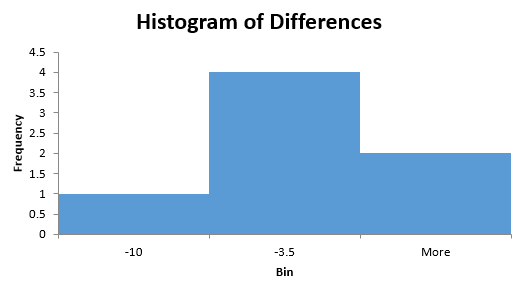
\includegraphics[width=6cm]{Figures/fig1.png}
		\vspace{-10 pt}
	\end{figure}
	
	We see nothing to be concerned here. So we conclude that the distribution of differences appear to have come from normal populations.
	\item Each pair was selected randomly since all 7 students were selected randomly.
	\item Since there are more than 70 ($= 10 \times n$) students taking Mintaek's class (in fact, there are 116 this semester), the population size ($N$) is larger than 10 times the sample size.
\end{itemize}
Since all conditions are met, we can use the matched paires t-test to make an inference on $\mu_D$ (population difference between two exam scores).

\noindent \textbf{Step 3}: We can now find the t-test statistic value and corresponding p-values. 

For $df = 7 - 1 = 6$, we find
\begin{align*}
t &= \dfrac{\bar{x}_D - \mu_D}{s_D / \sqrt{n}} 
= \dfrac{-4.42857 - 0}{5.12696 / \sqrt{7}}
= \dfrac{-4.42857}{1.93781}
= -2.29
\end{align*}
where $\mu_D$ is the hypothesized population mean difference from the hypotheses (or ``the null hypothesis value'').

At the t-distribution table, look at the row corresponding to $df = 6$. We can see that the positive value of our t-test statistic $t = 2.29$ is between 1.943 and 2.447. Note that I am using the positive value of $t$. It is because the t-distribution is symmetric. It means the tail area to the right of $t = 2.29$ (upper tail area) is going to be the same as the tail area to the left of $t = -2.29$ (lower tail area). 

Since the upper tail probability $p$ corresponding to $t = 1.943$ and $t = 2.447$ are 0.05 and 0.025, respectively, we can guess that the \textbf{upper} tail probability $p$ corresponding to our t-test statistic $t = 2.29$ is between 0.05 and 0.025. Therefore, the \textbf{lower} tail probability $p$ corresponding to our t-test statistic $t = -2.29$ is also between 0.05 and 0.025.

Since this is a two-sided test, our P-value would be between $2 \times 0.05$ and $2 \times 0.025$, that is 0.1 and 0.05. We can express our P-value as: $0.05 <$ P-value $< 0.1$.

For homework, you can use \url{surfstat.anu.edu.au/surfstat-home/tables/t.php} to find the exact P-value. Make sure to choose the correct graph corresponding to the tail you are interested in. Based on the output shown on the next page, we find the exact P-value of 0.0619. See the last page of Handout 2 for more information. Note that you will not be able to use this website for the exam, so it is important that you understand the process explained in the previous page.

\begin{figure}[!h]
	\centering
	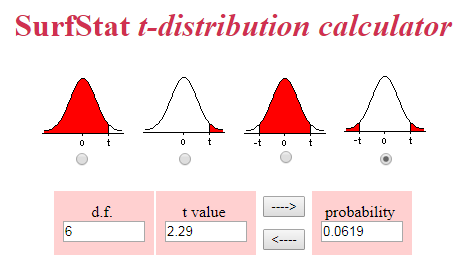
\includegraphics[width=9.25cm]{Figures/fig2.png}
	\vspace{-5 pt}
\end{figure}

\noindent \textbf{Step 4}: We fail to reject the null hypothesis under the significance level $\alpha = 0.05$. It is because our P-value was larger than our pre-determined significance level (0.05). We do not have a significant evidence to suggest that the difference in exam scores is not 0.

\noindent \textbf{Interpretation of the p-value}: The probability of obtaining a sample mean difference this far (or farther) away from 0 is 0.0619 if the population mean difference was 0. That is, there is 6.19\% chance of obtaining a sample mean difference of larger than 4.42857 OR smaller than -4.42857 if the true mean difference was 0 ($= H_0$ was true). Since the chance is greater than $\alpha = 0.05$, this would not be a surprising enough result to reject $H_0$.

\pagebreak

\textbf{IF THIS WAS A ONE-SIDED TEST WHERE} $\mathbf{H_A: \boldsymbol\mu_D < 0}$

\vspace{10 pt}

\noindent \textbf{Step 1}: $H_0$ is the same, just $H_A$ needs to be changed.
\begin{itemize}
	\item $H_0$: $\mu_D = 0$, population mean difference in exam scores is 0.
	\item $H_A$: $\mu_D < 0$, population mean difference in exam scores is less than 0. In other words, since $\mu_D = \mu_1 - \mu_2 < 0 \implies \mu_1 < \mu_2$, students did better in Exam 2 than Exam 1.
\end{itemize}

\noindent \textbf{Step 2}: Same

\noindent \textbf{Step 3}: Since $t = -2.29$ for $df = 6$, we find the \textbf{lower} tail area to be between 0.05 and 0.025. We are only interested in the lower tail since the sign in the $H_A$ is $<$. We do not consider the upper tail area. Therefore, our P-value would just be $0.025 <$ P-value $< 0.05$.

Similarly, for the website, choose the second graph from the left instead to find the area of only one tail. You should find the exact P-value of 0.031.

\noindent \textbf{Step 4}: We reject the null hypothesis under the significance level $\alpha = 0.05$. It is because our P-value was smaller than our pre-determined significance level. We have significant evidence to suggest that the difference in exam scores is less than 0. That is, the average exam 1 score is lower than the average exam 2 score, because $\mu_D = \mu_{exam1} - \mu_{exam2} < 0$ (the alternative hypothesis) would imply $\mu_{exam1} < \mu_{exam2}$.

\noindent \textbf{Interpretation of the p-value}: The probability of obtaining a sample mean difference of -4.42857 or lower is 0.031 if the population mean difference was 0. That is, there is 3.1\% chance of obtaining a sample mean difference of smaller than -4.42857 if the true mean difference was 0 ($= H_0$ was true). Since the chance is less than $\alpha = 0.05$, this would be a surprising enough result to reject $H_0$.

\pagebreak

\begin{example} Confidence intervals for paired (dependent) samples \\
	Mintaek now wants to estimate the true (or population) difference between the average \mbox{exam 1} scores and the average exam 2 scores with the 95\% certainty.
\end{example}
	
Technically, you still would need to check all conditions for the paired t-confidence intervals. However, you may notice that they are identical to ones for the matched pairs t-test. It will be omitted here for the sake of space.

We first find the standard error: $SE = \dfrac{s_D}{\sqrt{n}} = \dfrac{5.12696}{\sqrt{7}} = 1.93781$. 

We need to find the t critical value, $t^*$, to find the margin of error. Note that $df = 6$ and confidence level is 95\%. So we look at the row corresponding to $df = 6$ on the t-distribution table. We then find a column corresponding to the confidence level 95\% from the last row. You should find $t^* = 2.447$ as appropriate critical value.

When you want to find $t^*$ for $df$'s not listed on the t-distribution table, such as $df = 65$, you can use \url{surfstat.anu.edu.au/surfstat-home/tables/t.php} to find the $t^*$. Make sure to choose the third graph from the left to find the t critical values. Based on the output shown, we find the $2.447$ as our $t^*$ also. To get this value, enter 6 under d.f. and 0.95 under probability, then hit the $<$- - - - button

\begin{figure}[!h]
	\centering
	\vspace{-10 pt}
	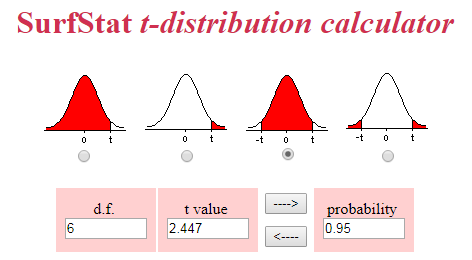
\includegraphics[width=9.25cm]{Figures/fig3.png}
	\vspace{-10 pt}
\end{figure}

Margin of error is defined as: $t^* \times SE = t^* \dfrac{s_D}{\sqrt{n}} = 2.447 \times 1.93781 = 4.742$. Then, we can finally calculate the 95\% confidence interval for the true (or population) difference between the average exam 1 scores and the average exam 2 scores.
\begin{align*}
\bar{x_D} \pm t^* \dfrac{s_D}{\sqrt{n}} = -4.43857 \pm 2.447 \times 1.93781 = -4.439 \pm 4.742 = (-9.18, 0.30)
\end{align*}

This means that we are 95\% certain/sure/confident that the interval (-9.18, 0.30) contains $\mu_D$, population mean difference between Exam 1 scores and Exam 2 scores.

\pagebreak

\begin{example} Hypothesis testing for independent (not paired) samples \\
	Mintaek is interested in finding out whether the average wingspan of Canada geese in the Julia Davis Park is the same with the average wingspan of Canada geese in the Ann Morrison Park. Mintaek captured 11 geese in the Julia Davis Park and another 11 geese in the Ann Morrison Park and measured wingspans of each one of them.
	\begin{table}[!h]
		\centering
		\begin{tabular}{llllllllllll}
			Julia Davis Park & 56 & 57 & 57 & 58 & 59 & 59 & 60 & 60 & 61 & 62 & 63 \\
			Ann Morrison Park & 57 & 58 & 58 & 59 & 60 & 61 & 63 & 64 & 64 & 65 & 65
		\end{tabular}
	\end{table}
\end{example}

\vspace{-10mm}
We can find the summary information for the data by using software.
\begin{table}[!h]
	\centering
	\begin{tabular}{l|lll}
		Julia Davis Park  & $n_1 = 11$ & $\bar{x}_1 = 59.272727$ & $s_1 = 4.818181$ \\ \hline
		Ann Morrison Park & $n_2 = 11$ & $\bar{x}_2 = 61.272727$ & $s_2 = 9.218181$
	\end{tabular}
\end{table}

\vspace{-10pt}
You first need to recognize that this is \textbf{NOT} a paired sample, and they are two independent samples. Although we would expect geese from two parks to be similar, you can't match one geese captured from the Julia Davis Park with one from the Ann Morrison Park. In that case, we need to use the two-sample t-test.

\noindent \textbf{Step 1}: Since the problem did not explicitly specify how much of a difference we want to see, any difference larger than 0 would suffice here. Admittedly, $\mu_0$ (null hypothesis value) would be 0 for most two sample problems.
\begin{itemize}
	\item $H_0$: $\mu_1 = \mu_2$ (or $\mu_1 - \mu_2 = 0$), population mean wingspan of geese in the Julia Davis Park is equal to the population mean wingspan of geese in the Ann Morrison Park.
	\item $H_A$: $\mu_1 \neq \mu_2$ (or $\mu_1 - \mu_2 \neq 0$), population mean wingspan of geese in the Julia Davis Park is not equal to the population mean wingspan of geese in the Ann Morrison Park.
\end{itemize}
Note that I let the geese in Julia Davis Park to be the Group 1 and geese in Ann Morrison Park to be Group 2. You can number your group the other way as long as you are consistent.

\noindent \textbf{Step 2}: We are using the two-sample t-test here because we have two samples that are independent (not individually paired). We check all the underlying conditions (See workbook page 152 for description of conditions). For the significance level, I will continue to use $\alpha = 0.05$. Unless otherwise stated, you should use $\alpha = 0.05$ for this class.

We check the following conditions for the two-sample t-test for means:
\begin{itemize}
	\item Since $n_1 + n_2 = 22 \geq 16$, we need to make sure that both sample graphs are not too skewed with no outliers. We can draw histograms of two samples.
	
	\begin{figure}[!h]
		\centering
		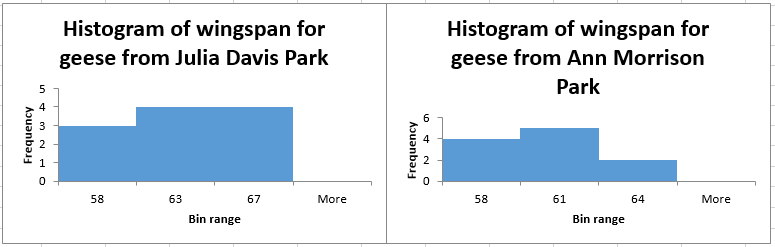
\includegraphics[width=15cm]{Figures/fig4.png}
		\vspace{-5 pt}
	\end{figure}
	
	Looking at the histograms shown on the next page, I have no concerns here and conclude that both sample graphs are not too skewed and have no outliers.
	\item Since we are not given whether geese were randomly captured, we would need to assume that geese in both parks were captured randomly.
	\item Population is certainly larger than 10 times the sample size. It is clear that there are more than 220 ($=10 (n_1 + n_2)=10 (11+11) = 10 \times 22$) geese in Boise.
\end{itemize}
Since all conditions are met, we can use the two-sample t-test to make an inference on difference between $\mu_1$ and $\mu_2$.

\noindent \textbf{Step 3}: We can now find the t-test statistic value and corresponding p-values.
\begin{align*}
t &= \dfrac{(\bar{x}_1 - \bar{x}_2) - \mu_0}{\sqrt{\frac{s_1^2}{n_1} + \frac{s_2^2}{n_2}}} = \dfrac{(59.272727 - 61.272727) - 0}{\sqrt{\frac{4.818181^2}{11} + \frac{9.218181^2}{11}}} = \dfrac{-2}{3.136149} = -1.77
\end{align*}
where $\mu_0$ (or $\mu_1 - \mu_2$) is the hypothesized population mean difference from the hypotheses (or ``the null hypothesis value'').

We find the $df$ for the two-sample t-test by taking $n_1 - 1$ or $n_2 - 1$, whichever is smaller. Here, we have $n_1 - 1 = 10$ and $n_2 - 1 = 10$, so the $df$ would be 10. Be careful, $n_1$ and $n_2$ can be different on other problems.

At the t-distribution table, look at the row corresponding to $df = 10$. We can see that the positive value of our t-test statistic $t = 1.77$ is between 1.372 and 1.812. Note that I am using the positive value of $t$ because t-distribution is symmetric. It means the tail area to the right of $t = 1.77$ is going to be the same as the tail area to the left of $t = -1.77$. 

Since the upper tail probability $p$ corresponding to $t = 1.372$ and $t = 1.812$ are 0.10 and 0.05, respectively, we can guess that the \textbf{upper} tail probability $p$ corresponding to our t-test statistic $t = 1.77$ is between 0.10 and 0.05. Therefore, the \textbf{lower} tail probability $p$ corresponding to our t-test statistic $t = -1.77$ is also between 0.10 and 0.05.

Since this is a two-sided test, our P-value would be between $2 \times 0.10$ and $2 \times 0.05$, that is 0.2 and 0.1. We can express our p-value as: $0.1 <$ P-value $< 0.2$.

For homework, you can use \url{surfstat.anu.edu.au/surfstat-home/tables/t.php} to find the exact P-value. Make sure to choose the correct graph corresponding to the tail you are interested in. The software gave me the exact P-value of 0.1072 for the two-sided tests.

\noindent \textbf{Step 4}: We fail to reject the null hypothesis. It is because our P-value was larger than our pre-determined significance level $\alpha = 0.05$. We do not have a significant evidence to suggest that the population mean wingspan of geese in the Julia Davis Park is not equal to the population mean wingspan of geese in the Ann Morrison Park.

\noindent \textbf{Interpretation of the p-value}: The probability of obtaining a sample mean difference this far (or farther) away from 0 is 0.1072 if the population mean difference was 0.

\vspace{10 pt}

\textbf{IF THIS WAS A ONE-SIDED TEST WHERE} $\mathbf{H_A: \boldsymbol\mu_1 < \boldsymbol\mu_2}$ \textbf{ OR } $\mathbf{\boldsymbol\mu_1 - \boldsymbol\mu_2 < 0}$

\vspace{10 pt}

\noindent \textbf{Step 1}: $H_0$ is the same, just $H_A$ needs to be changed.
\begin{itemize}
	\item $H_0$: $\mu_1 = \mu_2$ (or $\mu_1 - \mu_2 = 0$), population mean wingspan of geese in the Julia Davis Park is equal to the population mean wingspan of geese in the Ann Morrison Park.
	\item $H_A$: $\mu_1 < \mu_2$ (or $\mu_1 - \mu_2 < 0$), population mean wingspan of geese in the Julia Davis Park is less than the population mean wingspan of geese in the Ann Morrison Park.
\end{itemize}

\noindent \textbf{Step 2}: Same

\noindent \textbf{Step 3}: Since $t = -1.77$ for $df = 10$, we find the \textbf{lower} tail area of between 0.10 and 0.05. We are only interested in the lower tail. We do not consider the upper tail area. Therefore, our P-value would just be $0.05 <$ p-value $< 0.10$.

Similarly, for the website, choose the second graph from the left instead to find the area of only one tail. You should find the exact P-value of 0.0536.

\noindent \textbf{Step 4}: We reject the null hypothesis. It is because our P-value was smaller than our pre-determined significance level $\alpha = 0.05$. We have significant evidence to suggest that the population mean wingspan of geese in the Julia Davis Park is \textbf{less than} the population mean wingspan of geese in the Ann Morrison Park.

\noindent \textbf{Interpretation of the p-value}: The probability of obtaining a sample mean difference of -2 ($= \bar{x_1} - \bar{x_2}$) or lower is 0.0536 if the population mean difference was 0. 

\pagebreak

\begin{example} Confidence intervals for independent (not paired) samples \\
	Mintaek now wants to estimate the true (or population) difference between the population mean wingspan of geese in the Julia Davis Park and the population mean wingspan of geese in the Ann Morrison Park with the 95\% certainty.
\end{example}

Technically, you still would need to check all conditions for the two-sample t-confidence intervals. However, you may notice that they are identical to ones for the two-sample t-test. It will be omitted here for the sake of space.

We first find the standard error: $SE = \sqrt{\frac{s_1^2}{n_1} + \frac{s_2^2}{n_2}} = \sqrt{\frac{4.818181^2}{11} + \frac{9.218181^2}{11}} = 3.136149$. 

We need to find the t critical value, $t^*$, to find the margin of error. Note that $df = 15$ and confidence level is 95\%. So we look at the row corresponding to $df = 10$ on the t-distribution table. We then find a column corresponding to the confidence level 95\% from the last row. We should find $t^* = 2.228$ as appropriate critical value.

Margin of error is defined as: $t^* \times SE = t^* \sqrt{\frac{s_1^2}{n_1} + \frac{s_2^2}{n_2}} = 2.228 \times 3.136140 = 6.987$. Then we can finally calculate the 95\% confidence interval for the true (or population) difference between the population mean wingspan of geese in the Julia Davis Park and the population mean wingspan of geese in the Ann Morrison Park with the 95\% certainty.
\begin{align*}
(\bar{x}_1 - \bar{x}_2) \pm t^* \sqrt{\frac{s_1^2}{n_1} + \frac{s_2^2}{n_2}} &= -2 \pm 2.228 \times 3.136140 \\
&= -2 \pm 6.987 \\
&= (-2 - 6.987, -2+6.987) \\
&= (-8.99, 4.99)
\end{align*}
This means that we are 95\% certain/sure/confident that the interval (-8.99, 4.99) contains the difference between the population mean wingspan of geese in the Julia Davis Park and the population mean wingspan of geese in the Ann Morrison Park (which is just $(\mu_1 - \mu_2)$ in statistical terms).

\end{document}